\chapter{Introdução}
\label{cap:intro}

\section{Contextualização: a \textit{National Football League} e as posições ofensivas}

A \textit{National Football League} (NFL) é a principal liga de futebol americano do mundo. Composta por 32 franquias distribuídas entre as conferências AFC e NFC, a liga disputa 18 semanas de temporada regular seguidas de \textit{playoffs} e culmina no \textit{Super Bowl}, o evento esportivo mais assistido dos Estados Unidos. O modelo de negócio das franquias é ancorado na gestão de elenco: contratos multimilionários, \textit{trades} entre equipes e o \textit{NFL Draft} anual determinam o capital humano disponível para cada temporada.



O futebol americano é disputado entre duas equipes de 11 jogadores em campo, em um gramado de 100 jardas de comprimento (cerca de 91 metros), delimitado por duas zonas de pontuação (\textit{end zones}), uma em cada extremidade. O objetivo do time atacante é avançar a bola até a \textit{end zone} adversária; cada posse concede quatro tentativas (\textit{downs}) para avançar ao menos 10 jardas, sob pena de transferência da posse. Cada jogada se inicia a partir da linha de \textit{scrimmage}, linha imaginária que separa os times. A Figura~\ref{fig:campo_posicoes} ilustra o campo com as posições típicas do ataque e da defesa; QB, RB e WR aparecem destacados com borda dourada no diagrama elaborado pelo autor.

\begin{figure}[H]
  \centering
  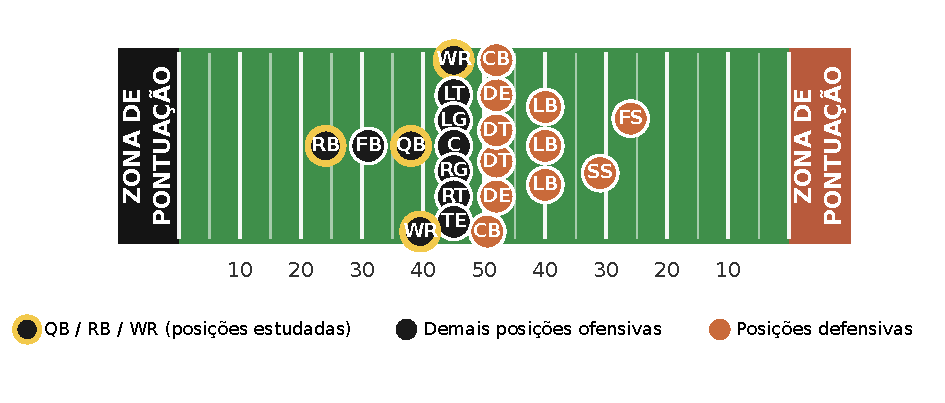
\includegraphics[width=\textwidth]{figuras/campo_posicoes_nfl.pdf}
  \caption[Campo de futebol americano com as posições ofensivas estudadas.]{Formação ofensiva típica em campo: QB, RB e WR em destaque (borda dourada); demais posições ofensivas em preto e defensivas em laranja.}
  \label{fig:campo_posicoes}
\end{figure}

As três posições ofensivas de habilidade estudadas neste trabalho, suas funções em campo e as principais métricas de desempenho associadas são descritas na Tabela~\ref{tab:posicoes_nfl}.

\begin{table}[H]
\centering
\caption{Posições estudadas (QB, RB e WR), com a função de cada uma em campo e as métricas de desempenho associadas.}
\label{tab:posicoes_nfl}
\renewcommand{\arraystretch}{1.75}
\footnotesize
\begin{tabular}{@{}p{2.3cm} p{5.2cm} p{6.2cm}@{}}
\toprule
\textbf{Posição} & \textbf{Função em campo} & \textbf{Principais métricas de desempenho} \\
\midrule
\textbf{Quarterback} (QB) &
Comandante do ataque. Recebe a bola no início de cada jogada (\textit{snap}), decide entre passar, entregar ao carregador (\textit{handoff}) ou correr. Concentra as decisões táticas ofensivas. &
\textit{Passer rating} (eficiência composta de passe), porcentagem de passes completados, jardas por tentativa de passe, razão de \textit{touchdowns} por tentativa (TD\%). \\
\addlinespace[10pt]
\textbf{Running Back} (RB) &
Principal carregador de bola. Avança pelo jogo terrestre (\textit{rushing}) após o \textit{handoff} do QB e pode atuar como receptor de passes curtos. Posição de alto desgaste físico. &
Jardas por carregada (YPC), total de \textit{touches} (carregadas + recepções), taxa de \textit{fumbles} (bolas perdidas após contato), participação no ataque terrestre da equipe. \\
\addlinespace[10pt]
\textbf{Wide Receiver} (WR) &
Principal receptor de passes. Alinhado nas extremidades da formação, realiza rotas predefinidas para se desmarcar da cobertura defensiva e receber passes do QB. &
Alvos recebidos (\textit{targets}), fatia dos alvos da equipe recebidos pelo jogador, taxa de recepção (\textit{catch rate}), jardas por alvo. \\
\bottomrule
\end{tabular}
\end{table}

A longevidade de carreira de um QB, RB ou WR impacta diretamente o planejamento esportivo e financeiro das equipes, tornando a modelagem estatística do tempo de permanência na liga um problema de relevância prática.


\needspace{8\baselineskip}
\section{Motivação e problema de pesquisa}
\label{sec:motivacao}

A longevidade de carreira na NFL é marcada por alta rotatividade: entre os jogadores ativos em 2025, o tempo médio de carreira é de 5,4 anos para QBs, 3,5 para WRs e 3,3 para RBs \citep{statista_nfl_career}, e muitos jogadores são cortados ou se aposentam antes de completar uma trajetória longa na liga. Para as equipes, isso pesa no planejamento esportivo e financeiro, porque renovar, estender ou encerrar um contrato depende de quanto tempo de carreira ainda se espera de cada jogador.

Essa decisão é tomada ao fim de cada temporada pelo gerente geral (\textit{general manager}, responsável pela gestão do elenco), com base no que o jogador mostrou até ali: o desempenho, o espaço que ocupa no ataque, as ausências e o lugar no elenco. Esses sinais mudam de uma temporada para outra, e uma mesma queda de produção pode ter peso diferente para um QB, um RB ou um WR.

Daí surgem duas perguntas práticas. A primeira é quais desses sinais acompanham a saída da liga em cada posição. A segunda é quanto tempo de carreira ainda resta a um jogador, dado o que se sabe dele ao fim de uma temporada. Responder a elas exige lidar com carreiras que ainda não terminaram e com informações que se renovam a cada ano, o que faz da análise de sobrevivência o caminho natural, apresentado no Capítulo~\ref{cap:metodologia}.


\needspace{8\baselineskip}
\section{Revisão de literatura}

Métodos quantitativos já foram aplicados a carreiras em vários esportes. No beisebol, \citet{bradbury2010} analisou os jogadores como ativos econômicos e a relação entre idade e desempenho. Na NBA, \citet{staw1995} usaram um modelo de risco com desempenho anual e encontraram mais risco de saída da liga para os escolhidos mais tarde no \textit{draft}, mesmo com o desempenho controlado. Na NFL, \citet{ducking2015} estimaram modelos de duração com desempenho anual, sem QBs, para testar discriminação racial na saída, e \citet{navarro2017} encontraram carreiras mais curtas entre jogadores com concussão.

Entre os trabalhos revisados, nenhum acompanha QBs, RBs e WRs com informações atualizadas a cada temporada e, ao mesmo tempo, procura entender o que se associa à saída e estimar o tempo de carreira restante. Este trabalho faz isso: acompanha QBs, RBs e WRs na mesma base, temporada a temporada; usa a parte inferencial para entender quais características acompanham a saída em cada posição; e usa a parte preditiva para estimar o tempo restante de carreira de cada jogador.


\needspace{8\baselineskip}
\section{Objetivos}

\subsection*{Objetivo geral}

Neste trabalho, o objetivo geral é caracterizar os fatores associados à longevidade de carreira de \textit{quarterbacks} (QB), \textit{running backs} (RB) e \textit{wide receivers} (WR) na NFL no período de 2012 a 2024, por meio de análise exploratória de dados e modelos inferenciais de sobrevivência com covariáveis dependentes do tempo, e estimar o tempo de carreira restante a partir do retrato de cada temporada, com validação temporal.

\subsection*{Objetivos específicos}

\begin{enumerate}
  \item Construir um painel de sobrevivência no formato \textit{counting process} (\textit{start--stop}) com covariáveis atualizadas anualmente para cada posição.
  \item Conduzir análise exploratória comparativa entre QB, RB e WR, com curvas de Kaplan--Meier e fatores descritivos da longevidade.
  \item Ajustar o modelo de Cox com covariáveis dependentes do tempo por posição.
  \item Verificar o pressuposto de riscos proporcionais por meio do teste de resíduos de Schoenfeld e identificar violações por posição.
  \item Ajustar o modelo aditivo de Aalen por posição e interpretar os coeficientes acumulados $B_j(t)$ como acréscimo de risco ao longo da carreira.
  \item Ler o Cox e o Aalen como abordagens complementares e, quando parte das covariáveis viola a proporcionalidade, ajustar o modelo híbrido de Cox--Aalen.
  \item Estimar o tempo de carreira restante por posição, comparando Kaplan--Meier, Cox penalizado, GBSA e RSF sob validação \textit{walk-forward}, com hiperparâmetros escolhidos por busca aninhada. Como análise complementar, avaliar o \textit{landmarking}.
\end{enumerate}


\needspace{5\baselineskip}
\section{Estrutura do trabalho}

O Capítulo~\ref{cap:metodologia} reúne a teoria dos métodos; o Capítulo~\ref{cap:material} descreve os dados, a construção do painel e a análise exploratória; os Capítulos~\ref{cap:resultados} e~\ref{cap:resultados_preditivos} apresentam os resultados inferenciais e preditivos; o Capítulo~\ref{cap:discussao} os cruza por posição; e o Capítulo~\ref{cap:conclusao} conclui, com as limitações e os trabalhos futuros. Os apêndices trazem os detalhes dos dados (Apêndice~\ref{apx:cap_dados}), da inferência (Apêndice~\ref{apx:cap_inferencia}) e da predição (Apêndice~\ref{apx:cap_predicao}).
